\section{The master rate formula}\label{sec:8.2}

A dark-matter particle that scatters in silicon, a dark photon of a few eV that is absorbed in it, and an excited dark-matter state that drops to its ground state on the way through all probe one property of the crystal: how readily it takes up a momentum $\vect{q}$ together with an energy $\omega$. For scattering through several target operators at once, \cref{eq:4.2-rate} already answers it, for one dark-matter particle of fixed velocity and for potentials that are plain numbers. Three things are missing before it can serve every model of \cref{sec:8.1}. The potentials are matrices in the spin space of the dark matter, and the rate needs the trace $\mathfrak{D}_{ab}$ of \cref{eq:8.1-D}. The halo supplies a distribution of velocities, and experiments quote rates per unit target mass. And absorption, in which the dark matter disappears, and the transitions in which the target gives energy away, look at first sight like different processes. We will see that all of them follow from one golden-rule calculation and land in different regions of the $(\vect{q}, \omega)$ plane (\cref{fig:8-plane}). The formula is exact in the target and first order in the coupling to the dark matter.

\subsection{Scattering}\label{sec:8.2-scattering}

Take a dark-matter particle in the plane wave $\vect{p} = \mchi\vect{v}$, in spin state $s$, and a target in the eigenstate $|i\rangle$. By \cref{eq:8.1-Hint} the amplitude to reach $\vect{p} - \vect{q}$, spin $s'$ and $|f\rangle$ is $\Vol^{-1}\sum_b\langle s'|\tilde V_b|s\rangle\langle f|O_b(\vect{q})|i\rangle$. The golden rule squares it, the spin sums turn the product of two potentials into the trace of \cref{eq:8.1-D}, the thermal average weights $|i\rangle$ with $p_i$, and the sum over final dark-matter momenta becomes $\Vol\int\dd^3q/(2\pi)^3$, as in \cref{sec:2.5}. Each step is written out in \cref{app:D.25}. The target then enters through the response matrix \cref{eq:4.2-Sab}, and the dark matter through $\mathfrak{D}_{ab}$:
\begin{keyresult}[Master rate formula: scattering]
\begin{equation}
  \varGamma(\vect{v}) = \int\frac{\dd^3q}{(2\pi)^3}\sum_{a,b}\underbrace{\mathfrak{D}_{ab}(\vect{q},\vect{v})}_{\text{coupling}}\,\underbrace{S_{ab}(\vect{q},\omega_{\vect{q}})}_{\text{target}} ,
  \label{eq:8.2-rate}
\end{equation}
the rate of one dark-matter particle of velocity $\vect{v}$, with $\omega_{\vect{q}}$ of \cref{eq:1.3-omegaq}, and per unit target mass
\begin{equation}
  \begin{split}
  \frac{\dd\mathcal{R}}{\dd\omega} &= \frac{1}{\rho_T}\,\underbrace{\frac{\rho_\chi}{\mchi}\int\dd^3v\,f_\chi(\vect{v})}_{\text{halo}}\int\frac{\dd^3q}{(2\pi)^3}\sum_{a,b}\underbrace{\mathfrak{D}_{ab}(\vect{q},\vect{v})}_{\text{coupling}} \\
  &\qquad\times\underbrace{S_{ab}(\vect{q},\omega)}_{\text{target}}\,\underbrace{\delta(\omega - \omega_{\vect{q}})}_{\text{kinematics}}
  \end{split} .
  \label{eq:8.2-spectrum}
\end{equation}
The rows $a, b$ run over the target operators of every species (\cref{eq:8.1-rows}), the target is in thermal equilibrium at temperature $T$, and $\omega$ takes either sign.
\end{keyresult}
\noindent The integrand is a contraction of two Hermitian positive semidefinite matrices, $\mathfrak{D}$ from the dark-matter side and $S$ from the target, and is therefore never negative. For potentials without dark-matter spin it is the rate \cref{eq:4.2-rate}, and for the density row alone it is \cref{eq:2.5-golden}. In the same form, Trickle, Zhang and Zurek write the scattering rate with an operator-valued potential~\cite[Eq.~(1)]{trickle2022effective}, and Trickle and collaborators write the total rate per unit target mass~\cite[Eqs.~(14)--(16)]{trickle2020multichannel}, both for a target that starts in one eigenstate.

The order of the indices matters once both matrices are complex. Since the golden rule pairs the conjugated potential $\tilde V_a^\dagger$ with the conjugated operator $O_a^\dagger$, \cref{eq:8.2-rate} contracts $\mathfrak{D}_{ab}$ with $S_{ab}$, element by element, which is the trace $\Tr[\mathfrak{D}S^{\mathrm{T}}]$. Splitting each Hermitian matrix into a real symmetric and a real antisymmetric part, $\mathfrak{D} = \mathfrak{D}_{\mathrm{R}} + \ii\mathfrak{D}_{\mathrm{I}}$ and $S = S_{\mathrm{R}} + \ii S_{\mathrm{I}}$, the other order, $\Tr[\mathfrak{D}S]$, differs from it by $2\Tr[\mathfrak{D}_{\mathrm{I}}S_{\mathrm{I}}]$ (\cref{app:D.25}). The two agree whenever one of the matrices is real. They differ when both are complex: for instance, when an operator with an explicit $\ii$, such as $\mathcal{O}_3$ of \cref{tab:8-operators}, meets a target whose current--spin response has an imaginary antisymmetric part, as spin--orbit coupling produces.

\Cref{eq:8.2-spectrum} reduces exactly to the rates of \cref{chap:1}. For an interaction through the electron density alone, $\mathfrak{D}_{ab} = |\tilde V|^2$ for $a = b = n_e$ and zero otherwise, and the contraction is $|\tilde V(\vect{q})|^2S(\vect{q},\omega)$. With $\Delta_\chi = 0$ the delta function is that of \cref{eq:1.1-rate}, and the two formulas coincide term by term, including the normalization $\rho_\chi/\mchi\rho_T$; this is \cref{eq:A.8-rate}. For a structure factor that depends only on $q$, or after averaging it over the directions of $\vect{q}$, the velocity integral and the angular integral act on the delta function alone. They give $\eta(\vmin)/2q$ per unit $\dd^3q/(2\pi)^3$ (\cref{eq:A.8-eta}), and with $|\tilde V|^2 = \pi\sigmae\FDM^2/\mu_{\chi e}^2$ the result is \cref{eq:1.5-rate}. For a crystal $S_{ab}$ depends on the direction of $\vect{q}$, and the full velocity kernel is kept, as \cref{app:A.8} describes for the daily modulation.

\subsection{Assumptions of the formula}\label{sec:8.2-conditions}

The derivation uses four assumptions, and each can fail in a known place.

\emph{First Born approximation.} The interaction with the dark matter acts once. The next term in the amplitude passes through intermediate dark-matter states and is smaller by roughly the ratio of the scattering amplitude $|f| = \mu_{\chi T}|\tilde V|/2\pi$ (\cref{sec:2.2}) to the range of the potential~\cite[Chap.~6]{sakurai2017modern}. For the heavy dark photon of \cref{we:8-darkphoton}, at $\mchi = \SI{10}{MeV}$ and $m_V = \SI{30}{MeV}$, $|f|\,m_V = 2\times10^{-8}$. At the cross-sections used in this book the correction is below $10^{-4}$ for $\mchi$ from \SI{1}{keV} to \SI{1}{GeV} and $m_V$ up to \SI{10}{GeV} (\cref{lim:8.2a}). The interactions inside the target are not expanded at all: $S_{ab}$ is exact, and any approximation in it is an approximation to the target. \Cref{sec:8.5} records such approximations in a truncation label $\mathfrak{T}$, the list of orders that a calculation keeps in each small parameter of the target. No truncation of the target changes the master formula; it changes only $S_{ab}$.

\emph{Plane waves.} The halo is an incoherent mixture of momenta, distributed as $f_\chi$, and the final dark-matter state is not observed. Averaging plane-wave rates over $f_\chi$ is then exact. For bosons light enough that the halo is a classical wave, the ensemble average still holds for a long enough observation, and \cref{sec:8.2-absorption} gives the condition.

\emph{Gibbs target.} The target is in thermal equilibrium before each event, with the weights $p_i = \ee^{-\beta E_i}/\mathcal{Z}$. A detector qualifies when events are rare compared with its relaxation. A target prepared out of equilibrium, such as an ensemble of polarized nuclear spins, still obeys \cref{eq:8.2-rate} with its own populations in $S_{ab}$, provided its density operator is diagonal in energy, but detailed balance and the fluctuation--dissipation theorem then fail. The extension to a density operator with coherences between energy eigenstates, or to a target driven during the exposure, is open.

\emph{Unpolarized dark matter.} The halo has no preferred spin direction, which is what the factor $1/(2|\vect{S}_\chi| + 1)$ in $\mathfrak{D}_{ab}$ assumes. A polarized flux, with spin density matrix $\op{\varrho}_\chi$ of unit trace, has
\begin{equation}
  \mathfrak{D}_{ab}(\vect{q}, \vect{v}) = \Tr_\chi\bigl[\op{\varrho}_\chi\,\tilde V_a(\vect{q}, \bar{\vect{v}}_\chi)^\dagger\,\tilde V_b(\vect{q}, \bar{\vect{v}}_\chi)\bigr] ,
  \label{eq:8.2-polarized}
\end{equation}
which is \cref{eq:8.1-D} for $\op{\varrho}_\chi = 1/(2|\vect{S}_\chi| + 1)$.

\begin{limitbox}[First Born approximation for a Yukawa potential][lim:8.2a]
For a Yukawa potential of strength $y_\chi y_T$, with $y_T = y_e$ for an electron and $Ay_N$ for a nucleus, and range $1/m_V$, the second Born term changes the cross-section by the fraction
\begin{equation}
  \delta_{\mathrm{Born}} \simeq \pm\frac{\mu_{\chi T}\,y_\chi y_T}{2\pi(m_V + p_{\mathrm{rel}})} = \pm|f(0)|\,m_V\,\frac{m_V}{m_V + p_{\mathrm{rel}}} ,
  \label{eq:8.2-born}
\end{equation}
upper sign for attraction~\cite[Chap.~6]{sakurai2017modern}. At $p_{\mathrm{rel}} \ll m_V$ it is exact: the zero-energy radial equation gives the scattering length $a = a_{\mathrm{Born}}(1 \pm |f(0)|m_V/2)$. At $p_{\mathrm{rel}} \gg m_V$, partial waves give a correction below $y_\chi y_T/4\pi v$ at every $q \le 2p_{\mathrm{rel}}$ (0.28 of it at $q = 2p_{\mathrm{rel}} = 20\,m_V$), falling as $m_V/p_{\mathrm{rel}} \to 0$, where the Born cross-section of the Coulomb potential is exact; \cref{eq:8.2-born} then overestimates it.
\par\smallskip
{\centering
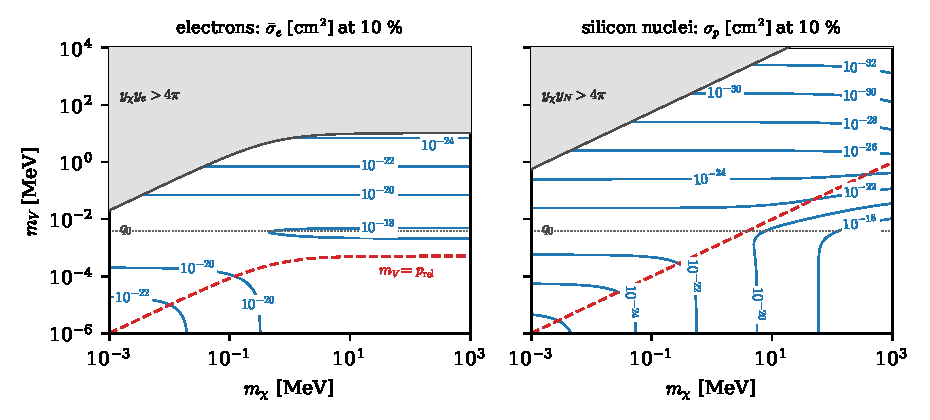
\includegraphics[width=\linewidth]{figures/ch08/limit8_2a.pdf}
\captionof{figure}{Cross-section at which $|\delta_{\mathrm{Born}}|$ of \cref{eq:8.2-born} reaches 0.1, against $\mchi$ and $m_V$, at $v = 10^{-3}$. Left: electrons, $\sigmae$ with the form factor normalized at $q_0 = \alpha m_e$ (\cref{eq:1.4-yukawa-sigma}). Right: silicon nuclei, coherent ($A = 28$), $\sigma_p$ normalized in the same way. With the coupling fixed by the cross-section, $\mchi$ enters only through $p_{\mathrm{rel}} = \mu_{\chi T}v$ (dashed, $m_V = p_{\mathrm{rel}}$; dotted, $m_V = q_0$). Gray: the \SI{10}{\percent} point needs $y_\chi y_e$ or $y_\chi y_N$ above $4\pi$, which happens for $m_V + p_{\mathrm{rel}} > 20A\mu_{\chi T}$ ($A = 1$ for electrons). At $\sigmae = \SI{e-37}{cm^2}$ and $\sigma_p = \SI{e-40}{cm^2}$ the largest correction in the plot is $4.5\times10^{-5}$ and $8.0\times10^{-5}$, at $m_V = \SI{10}{GeV}$. With perturbative couplings, \SI{10}{\percent} needs $\sigmae \ge \SI{4.9e-25}{cm^2}$ (at $m_V \approx \SI{10}{MeV}$) and $\sigma_p \ge \SI{1.6e-34}{cm^2}$ (at $\mchi = \SI{1}{GeV}$, $m_V = \SI{10}{GeV}$).}\label{fig:8-born-limit}
\par}
\smallskip
A correction of order one needs couplings near $4\pi$ with $m_V \lesssim 20A\mu_{\chi T}$, where the attractive potential binds and the cross-section has resonances that only the full partial-wave solution describes.
\end{limitbox}

\subsection{Absorption of a bosonic field}\label{sec:8.2-absorption}

A boson $\phi$ of mass $m_\phi$ that is absorbed leaves nothing behind, and its whole energy and momentum go into the target. By \cref{sec:8.1-absorption} its coupling is linear in the field and turns each target bilinear into a row at $\vect{q} = \vect{p}_\phi$. We write the coefficient of row $a$ per unit field amplitude as $g^\phi_a$, so that for the scalar of \cref{eq:8.1-scalar}, $g^\phi_{n_e} = -g_{\phi ee}$ and $g^\phi_{\mathcal{T}_e} = g_{\phi ee}/m_e$. For a vector field the polarization vector of the absorbed quantum sits inside $g^\phi_a$. Quantize the field in the box, with quanta of energy $\omega_\phi = m_\phi(1 + v^2/2)$. The matrix element that removes one quantum from a mode with $N_\phi$ quanta is $\sqrt{N_\phi/2\omega_\phi \Vol}\,\sum_bg^\phi_b\langle f|O_b(\vect{p}_\phi)|i\rangle$, and the golden rule, summed over $f$ and averaged over $i$, gives the response matrix again (\cref{app:D.25}). Per absorbed particle,
\begin{keyresult}[Master rate formula: absorption]
\begin{equation}
  \begin{gathered}
  \varGamma_{\mathrm{abs}} = \frac{1}{2\omega_\phi}\sum_{a,b}\underbrace{g^{\phi\,*}_a\,g^\phi_b}_{\text{coupling}}\,\underbrace{S_{ab}(\vect{p}_\phi,\omega_\phi)}_{\text{target}}, \\
  \varGamma_{\mathrm{net}} = (1 - \ee^{-\beta\omega_\phi})\,\varGamma_{\mathrm{abs}} = -\frac{1}{\omega_\phi}\,\Imag\sum_{a,b}g^{\phi\,*}_a\,g^\phi_b\,R_{ab}(\vect{p}_\phi,\omega_\phi) ,
  \end{gathered}
  \label{eq:8.2-abs}
\end{equation}
with $\omega_\phi \simeq m_\phi$. The event rate per unit target mass is $(\rho_\chi/m_\phi\rho_T)\langle\varGamma_{\mathrm{abs}}\rangle$, averaged over the directions and magnitudes of $\vect{p}_\phi = m_\phi\vect{v}$ with $f_\chi$.
\end{keyresult}
\noindent The absorption rate is the scattering formula evaluated at a single point, with $\mathfrak{D}_{ab}$ replaced by $g^{\phi\,*}_ag^\phi_b/2\omega_\phi$. The factor $1/2\omega_\phi$ is the relativistic normalization of one quantum. The number of quanta per unit volume, $\rho_\chi/m_\phi$, sets the event rate, not their flux: the speed of the dark matter enters only through the small momentum $\vect{p}_\phi$, as \cref{sec:2.1} found for a classical field.

The two rates in \cref{eq:8.2-abs} answer different questions. $\varGamma_{\mathrm{abs}}$ counts the quanta the target absorbs, each depositing $\omega_\phi$, and it is what a detector records. The field also stimulates the target to emit quanta into the occupied modes, at the rate $\ee^{-\beta\omega_\phi}\varGamma_{\mathrm{abs}}$ by detailed balance, and such an event takes energy out of the target. $\varGamma_{\mathrm{net}}$ is the difference, the rate at which the field loses quanta, and the fluctuation--dissipation theorem \cref{eq:4.2-fdt} writes it through the imaginary part of the response. That is the form in which Mitridate and collaborators state absorption, as the imaginary part of the self-energy of $\phi$, $\varGamma = -\Imag\Pi_{\phi\phi}/\omega$~\cite[Eqs.~(20)--(22)]{mitridate2021dark}, with $\Pi_{\phi\phi} = \sum_{ab}g^{\phi\,*}_ag^\phi_bR_{ab}$ in our normalization. For $\omega_\phi$ of an eV in a detector at \SI{10}{mK}, however, $\ee^{-\beta\omega_\phi}$ is zero for every purpose, and the two rates coincide.

The number of quanta in a volume $(1/m_\phi v)^3$ is $\rho_\chi/(m_\phi^4v^3)$, which exceeds one for $m_\phi$ below about \SI{7}{eV} at $v = 10^{-3}$, and grows as $m_\phi^{-4}$ below. Lighter bosons form a classical field rather than a gas of particles. The quantized calculation still applies, because the rate is linear in $N_\phi$ and the difference between $N_\phi$ and $N_\phi + 1$ in the emission matrix element, the spontaneous emission that a classical field lacks (\cref{sec:2.1}), is negligible. The same rate also follows from the classical field directly. Its amplitude is a sum of many modes with random phases, and by the central limit theorem it is a Gaussian random field. Averaging the transition probability over this Gaussian ensemble, the \emph{Gaussian field average}, removes the cross terms between different modes and leaves $\langle|\phi_{\vect{k}}|^2\rangle$ for each mode, which the energy density fixes; \cref{app:D.25} shows that the result is \cref{eq:8.2-abs} term by term.

The ensemble average needs an observation time long compared with the shorter of the coherence time $t_{\mathrm{coh}}$ of the field, of order $1/m_\phi v_0^2$, about \SI{1}{ns} at $m_\phi = \SI{1}{eV}$, and the inverse width of the target's response; a single record reproduces it only when it is also long compared with $t_{\mathrm{coh}}$. When both times exceed the record, for a field of neV mass or below acting on a sharp resonance such as a nuclear spin, the field drives the target coherently. The transition amplitude rather than the probability then grows linearly in time, and the golden rule gives way to the coherent classical-field treatment of \cref{sec:14.6}.

\Cref{eq:8.2-abs} reduces exactly to the dark-photon rate \cref{eq:1.4-dp-abs}. A dark photon at rest couples to the current of the electrons with strength $\zeta e$ times its polarization $\hat{\vect{e}}$ (\cref{sec:8.1-absorption}), and the only row is $\hat{\vect{e}}\cdot\vect{j}_e$, with $g^\phi = \zeta e$. With the proper current response $\tilde R^{\mathrm{T}}_{jj}$ of \cref{sec:4.4}, \cref{eq:8.2-abs} gives $\varGamma_{\mathrm{net}} = -(\zeta^2e^2/m_\phi)\Imag\tilde R^{\mathrm{T}}_{jj}(m_\phi)$. The diamagnetic term of the current is real and does not contribute. By the transverse dielectric function of \cref{sec:4.4}, $\varepsilon_2 = -(e^2/\omega^2)\Imag\tilde R^{\mathrm{T}}_{jj}$, and with $\sigma_1 = \omega\varepsilon_2$ (\cref{eq:4.4-sigma}) the rate is $\zeta^2\sigma_1(m_\phi)$, the same for every polarization in a cubic crystal (\cref{eq:4.4-ET}). The full response also contains the chain in which the induced current radiates an ordinary photon that the target absorbs again. Summing it, \cref{app:D.25} shows that it turns $\zeta^2$ into $\zeta_{\mathrm{eff}}^2$ of \cref{sec:1.4}. Multiplying by $\rho_\chi/m_\phi\rho_T$ gives \cref{eq:1.4-dp-abs}.

Fermionic absorption (\cref{sec:8.1-absorption}) fits the same formula. The dark matter disappears and a light fermion $\tilde\nu$ leaves with momentum $\vect{p} - \vect{q}$. The sum over final dark-matter momenta that produced \cref{eq:8.2-rate} becomes the sum over the momenta of $\tilde\nu$, and energy conservation sets $\omega$ to \cref{eq:8.1-omega}, which is $\mchi - q$ for a massless $\tilde\nu$. The rows and $S_{ab}$ are those of scattering, now sampled along a line at $q \approx \mchi$. Only $\mathfrak{D}_{ab}$ changes: the spinors of the relativistic $\tilde\nu$ enter it with relativistic normalization, which \cref{sec:10.9} constructs.

\subsection{Negative energies and exothermic dark matter}\label{sec:8.2-exothermic}

The master formula holds for either sign of $\omega$. The kinematics of scattering allows it to be negative: a dark-matter particle that moves against $\vect{q}$, or that recoils with more kinetic energy than it brings, gains energy, $\omega_{\vect{q}} < 0$. Whether such a transfer happens is decided by the target alone. At $T = 0$ the target starts in its ground state, $S_{ab}(\vect{q},\omega)$ vanishes for $\omega < 0$, and the half-plane below the axis in \cref{fig:8-plane} is closed. A warm target opens it, with the weight fixed by detailed balance. In matrix form, $S_{ab}(-\vect{q},-\omega) = \ee^{-\beta\omega}S_{ba}(\vect{q},\omega)$ (\cref{sec:4.2}), so a transfer of $\omega < 0$ is suppressed relative to the reverse one by $\ee^{-\beta|\omega|}$, the Boltzmann factor of the excitation the target gives up. For an electronic excitation across the gap of silicon, this factor is smaller than any power of the temperature, and an expansion in the phonon occupations (the thermal order $n_T$ of \cref{sec:8.5}) drops it at every order. For a phonon it is the occupation $n_{\vect{Q}\nu}$ itself: the negative-$\omega$ part of a one-phonon rate is proportional to $n_{\vect{Q}\nu}$, of first order in the occupations. The same holds for absorption, whose emission partner sits at the point $(-\vect{p}_\phi, -\omega_\phi)$.

Exothermic dark matter does something different: it does not reweight the band, it moves it. A particle that arrives in an excited state and leaves in the lower one, with $\Delta_\chi < 0$, adds $|\Delta_\chi|$ to every $\omega_{\vect{q}}$ of \cref{eq:1.3-omegaq}. The band of allowed $(\vect{q}, \omega)$ shifts up by $|\Delta_\chi|$, reaches $q \to 0$ at $\omega = |\Delta_\chi|$, and there looks like the absorption of a boson of mass $|\Delta_\chi|$, with $\vect{q}$ set by the velocity rather than fixed at $m_\phi\vect{v}$ (\cref{fig:8-plane}). Since the energy now comes from the dark matter, the target needs no temperature, and the response is sampled at positive $\omega$ even for the slowest particles. An endothermic splitting, $\Delta_\chi > 0$, shifts the band down, and part of it can then be reached only with energy taken from a warm target.

Detailed balance ties the two directions of each transition, for the dark matter as well as for the target. Let $\vect{p}$ and $\vect{p}'$ be two dark-matter states, of any masses, and $\omega = E(\vect{p}) - E(\vect{p}')$ the energy that the transition $\vect{p} \to \vect{p}'$ deposits. Then, for unpolarized dark-matter states of equal spin,
\begin{equation}
  \varGamma(\vect{p}' \to \vect{p}) = \ee^{-\beta\omega}\,\varGamma(\vect{p} \to \vect{p}') ,
  \label{eq:8.2-db}
\end{equation}
for the rate into one final momentum (\cref{app:D.25}). The reverse transition is driven by the conjugated interaction, which exchanges $\mathfrak{D}_{ab}$ for $\mathfrak{D}_{ba}$ and $O_b$ for $O_b^\dagger$, and the two exchanges cancel in the contraction; what remains is the ratio of the Gibbs weights of the two target states. The down-scattering of an exothermic particle, $\chi_2 \to \chi_1$, and the up-scattering $\chi_1 \to \chi_2$ that a warm target can drive are therefore one process read in two directions. A population of dark matter in contact with the target for long enough would relax to the temperature of the target.

\begin{figure}[tbp]
  \centering
  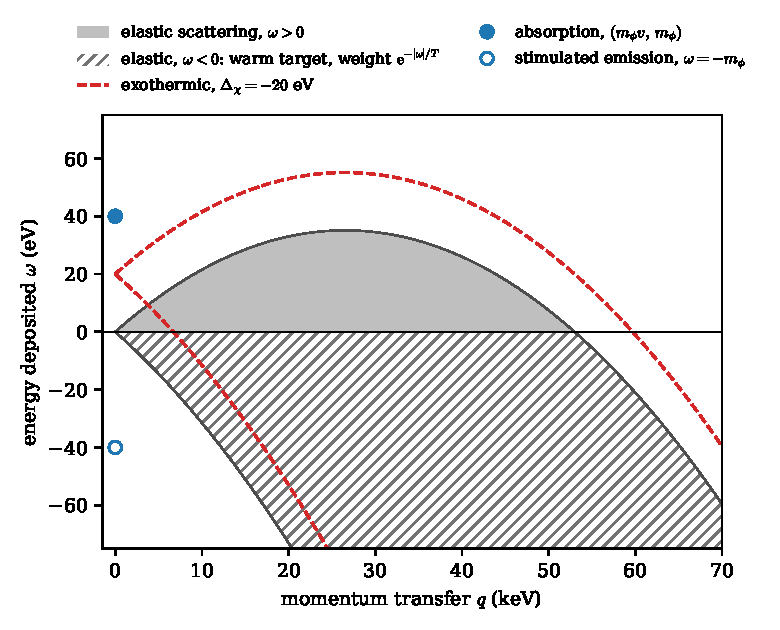
\includegraphics[width=0.9\linewidth]{figures/ch08/fig8_1.pdf}
  \caption{Where the master rate formula samples the response, in the plane of momentum transfer $q$ and energy deposited $\omega$, for $\mchi = \SI{10}{MeV}$ and speeds up to $v_{\mathrm{max}} = 2.650\times10^{-3}$. Elastic scattering reaches the band $-qv_{\mathrm{max}} - q^2/2\mchi \le \omega \le qv_{\mathrm{max}} - q^2/2\mchi$, the extreme values of $\omega_{\vect{q}}$ over all directions of $\vect{v}$. Its upper part (gray, $\omega > 0$, maximum \SI{35}{eV} at $q = \mchi v_{\mathrm{max}} = \SI{26.5}{keV}$) is open at any temperature. Its lower part (hatched, $\omega < 0$) is open only for a target at $T > 0$, with weight $\ee^{-|\omega|/T}$ relative to the reverse transfer. Exothermic dark matter with $\Delta_\chi = \SI{-20}{eV}$ shifts the band up by $|\Delta_\chi|$ (dashed). Absorption of a boson of mass $m_\phi = \SI{40}{eV}$ is a point at $q = m_\phi v \approx \SI{40}{meV}$, $\omega = m_\phi$ (filled circle); stimulated emission into the occupied field is the point $\omega = -m_\phi$ (open circle). Fermionic absorption with a massless outgoing fermion, $\omega = \mchi - q$, is a line at $q \approx \mchi$, far to the right.}
  \label{fig:8-plane}
\end{figure}

\subsection{Conditions for off-diagonal terms}\label{sec:8.2-cross}

The off-diagonal terms of the contraction are the part of a rate that no single-operator calculation contains. They need two things at once. The dark-matter side must couple two rows with a nonzero product $\mathfrak{D}_{ab}$, and the target must correlate the same two rows, $S_{ab} \neq 0$. Each factor vanishes for a reason of symmetry in the commonest cases. On the dark-matter side, a coefficient linear in $\vect{S}_\chi$ never interferes with one that is independent of it (\cref{sec:8.1}). On the target side, the density and the spin density of a target without magnetic order are uncorrelated, since $\Tr\boldsymbol{\sigma} = 0$. The worked example takes a target with magnetic order and a coupling that survives the trace over the dark-matter spin.

\begin{workedexample}{Density and spin couplings in a polarized electron gas}\label{we:8-cross}
Take the free electron gas at the valence density of silicon, $\nd_e = \SI{2.00e23}{cm^{-3}}$, fully polarized along $\hat{\vect{z}}$ by a uniform exchange field strong enough to lift the minority band above the Fermi level, a toy half-metal. All electrons have $S_z = +\frac12$ and fill one Fermi sphere of radius $k_{\mathrm{F}\uparrow} = 2^{1/3}k_{\mathrm{F}} = \SI{4.50}{keV}$, with $v_{\mathrm{F}\uparrow} = 8.80\times10^{-3}$ and $E_{\mathrm{F}\uparrow} = \SI{19.8}{eV}$; the exchange splitting must exceed $E_{\mathrm{F}\uparrow}$. We work at $T = 0$ with two rows, the density $n_e$ and the spin density $s^z_e$ of \cref{eq:8.1-rows}.

The Hamiltonian conserves the spin of each electron, so every state that $n_e$ or $s^z_e$ reaches from the ground state has all spins up, and on those states $s^z_e(\vect{q}) = \frac12 n_e(\vect{q})$ exactly. The response matrix is then
\begin{equation*}
  \begin{pmatrix} S_{nn} & S_{ns} \\ S_{sn} & S_{ss} \end{pmatrix} = S_\uparrow(\vect{q},\omega)\begin{pmatrix} 1 & \frac12 \\ \frac12 & \frac14 \end{pmatrix} ,
\end{equation*}
with $S_\uparrow$ the structure factor of one spin, half of \cref{eq:4.2-gas} with $k_{\mathrm{F}} \to k_{\mathrm{F}\uparrow}$. Its determinant vanishes: the two rows are one operator, and the matrix saturates the bound \cref{eq:4.2-positivity}. At $q = q_0 = \SI{3.73}{keV}$ and $\omega = \SI{5}{eV}$ we are in the linear region of the sphere, below $qv_{\mathrm{F}\uparrow} - q^2/2m_e = \SI{19.2}{eV}$, and $S_\uparrow = m_e^2\omega/2\pi q = \SI{5.57e7}{eV^2}$, half of the unpolarized gas at the same density.

For potentials $\tilde V_n$ and $\tilde V_s$ on the two rows, real and without dark-matter spin, the contraction is
\begin{equation*}
  \tilde V_n^2S_{nn} + 2\tilde V_n\tilde V_sS_{ns} + \tilde V_s^2S_{ss} = S_\uparrow\bigl(\tilde V_n + \tfrac12\tilde V_s\bigr)^2 .
\end{equation*}
Every electron carries $S_z = \frac12$, so a coupling to the spin acts as an extra density potential and adds to it in the amplitude. The sum of the two single-operator rates is $S_\uparrow(\tilde V_n^2 + \tilde V_s^2/4)$. It misses the term $\tilde V_n\tilde V_sS_\uparrow$, which is first order in the weaker coupling, and at $\tilde V_s = -2\tilde V_n$, where the true rate vanishes, it is wrong by the whole of $2\tilde V_n^2S_\uparrow$.

Which models produce such a $\tilde V_s$? The standard pair $\mathcal{O}_1$ and $\mathcal{O}_4 = \vect{S}_\chi\cdot\vect{S}_e$ does not: $\tilde V_s = c_4^{(e)}\vect{S}_\chi$, and the trace over the unpolarized dark-matter spin removes the cross term. A spin coupling free of $\vect{S}_\chi$ is $\mathcal{O}_7 = \vect{S}_e\cdot\vect{v}^\perp$, which reduces to $\bar{\vect{v}}_\chi\cdot\vect{s}_e - \mathcal{J}^{\alpha\alpha}_e$ (\cref{tab:8-operators}). No standard model produces $\mathcal{O}_7$ at leading order (\cref{sec:8.1}); we take it as the simplest spin coupling that survives the trace. Take it together with $\mathcal{O}_1$, with coefficients $c_1$ and $c_7$. The rows $s^x_e$, $s^y_e$, $\mathcal{J}^{xx}_e$ and $\mathcal{J}^{yy}_e$ flip the spin and reach states orthogonal to those of $n_e$, so the terms of first order in $c_7$ are
\begin{equation*}
  2c_1c_7\bigl[\bar v_{\chi,z}\,S_{ns} - S_{n\mathcal{J}}\bigr], \qquad
  S_{n\mathcal{J}} = \tfrac12\Bigl\langle\frac{(2\vect{k} + \vect{q})_z}{2m_e}\Bigr\rangle S_\uparrow ,
\end{equation*}
since the element of $\mathcal{J}^{zz}_e$ between $\vect{k}$ and $\vect{k} + \vect{q}$ is $\frac12(2\vect{k} + \vect{q})_z/2m_e$, and the brackets average over the pairs at this $(\vect{q},\omega)$. Since the pairs fill an annulus symmetric about $\vect{q}$ (\cref{we:8-O2}), the transverse part of $\vect{k}$ averages away, and $(2\vect{k} + \vect{q})\cdot\hat{\vect{q}}/2m_e = \omega/q$ for every pair. As a result, $S_{n\mathcal{J}} = \frac12(\omega/q)\hat q_zS_\uparrow$. On the dark-matter side, $\hat{\vect{q}}\cdot\bar{\vect{v}}_\chi = \omega/q$ for elastic scattering, so $\bar v_{\chi,z} = (\omega/q)\hat q_z + \vect{v}_{\mathrm{T}}\cdot\hat{\vect{z}}$, with $\vect{v}_{\mathrm{T}}$ the part of $\vect{v}$ transverse to $\vect{q}$. The longitudinal parts cancel, as \cref{eq:8.1-transverse} requires, and the integrand of \cref{eq:8.2-rate} becomes
\begin{equation*}
  c_1^2\,S_\uparrow + c_1c_7\,(\vect{v}_{\mathrm{T}}\cdot\hat{\vect{z}})\,S_\uparrow + O(c_7^2) .
\end{equation*}
For the dark matter of \cref{we:8-O2}, $\mchi = \SI{100}{MeV}$ and $v = 2.0\times10^{-3}$, $\vmin = 1.36\times10^{-3}$ and $v_{\mathrm{T}} = 1.47\times10^{-3}$. With $\vect{v}_{\mathrm{T}}$ along the magnetization, the cross term is $1.5\times10^{-3}\,c_7/c_1$ of the $\mathcal{O}_1$ rate. The rate of $\mathcal{O}_7$ alone is second order in $c_7$ and quadratic in the velocities. Its squared matrix elements, summed over the final spin, are $|\vect{v}^\perp|^2/4 \le (v_{\mathrm{max}} + v_{\mathrm{F}\uparrow} + q/2m_e)^2/4 = 5.7\times10^{-5}$, and its structure factors are at most $S_\uparrow$ and $m_ek_{\mathrm{F}\uparrow}^2/4\pi q = 4.0\,S_\uparrow$, the second for spin flips into the empty minority band, which an exchange splitting above $E_{\mathrm{F}\uparrow} + \omega$ closes; the bound is generous. At $c_7 = c_1$ the cross term is therefore at least five times the rate of $\mathcal{O}_7$ alone.

The cross term is odd in $\vect{v}_{\mathrm{T}}$. At fixed $\vect{q}$ the halo integral runs over the velocities with $\hat{\vect{q}}\cdot\vect{v} = \vmin$, and for the laboratory Maxwellian $f_\chi \propto \ee^{-|\vect{v} + \vect{v}_{\mathrm{E}}|^2/v_0^2}$ of \cref{app:A.8} the exponent splits into a longitudinal and a transverse Gaussian. Apart from the escape cut, the transverse Gaussian is centered on $-\vect{v}_{\mathrm{E},\mathrm{T}}$, the part of $-\vect{v}_{\mathrm{E}}$ transverse to $\vect{q}$, and the averaged cross term is $-c_1c_7\,(\vect{v}_{\mathrm{E},\mathrm{T}}\cdot\hat{\vect{z}})\,S_\uparrow$, at most $8.4\times10^{-4}\,c_7/c_1$ of the $\mathcal{O}_1$ rate for $|\vect{v}_{\mathrm{E}}| = \SI{250.5}{km.s^{-1}}$. It vanishes for an isotropic halo, follows the angle between the magnetization and the dark-matter wind, and changes sign when the magnetization is reversed.

A partially polarized gas has two spheres and $S_{ns} = \frac12(S_\uparrow - S_\downarrow)$. In the linear region, however, the structure factor of one spin, $m_e^2\omega/2\pi q$, does not depend on the radius of its sphere, and $S_{ns}$ vanishes there even though the gas is magnetized. At a polarization of 0.5 and $q = q_0$, $S_{ns} = 0$ at \SI{5}{eV}; at \SI{10}{eV}, where the minority sphere has left its linear region (its edge is at \SI{7.07}{eV}), $S_{ns}/S_{nn} = 0.068$.
\end{workedexample}

A cross term needs a coupling and a target that break the same symmetry, here time reversal, and when both do, it enters the rate at first order in the weaker coupling, where each single-operator rate enters at second order. How large it can be is fixed by positivity, and the polarized gas reaches the limit; \cref{sec:8.3} derives the bound together with the other relations that hold for every target.
